\input lec_preamble.tex

%% YOUR LOCAL MACROS AND PACKAGE GO HERE
\newcommand{\Expect}{\mathbb{E}}
\newcommand{\Prob}{\mathbb{P}}
\newcommand{\calF}{\mathcal{F}}
\newcommand{\calX}{\mathcal{X}}
\newcommand{\matx}{\ensuremath{\mathcal{X}}}
\def\PP{\mathbb{P}}
\newcommand{\matf}{\ensuremath{\mathcal{F}}}

%% SOME RULES
%% - only use pdfLaTeX to compile!!
%% - for aligned equations, use align, do NOT use eqnarray
%% - Use \| instead of ||, e.g., for divergence D(P\|Q), norms \|x\|_2
%% - for unreferenced displayed math, use \[\] and do not number them
%% - for labeling, use the following convention
%%          theorem: 			\label{thm:fermat}
%%          definition: 	\label{def:entropy}
%%          lemma: 				\label{lmm:fermat}
%%          proposition: 	\label{prop:fermat}, etc
%% - for bibliography use bibtex and add your entry to bibnotes.bib


%% lecture starts below
%% 1. lecture number (also name the file accordingly like lec01.tex)
%% 2. title (short summary of the content)
%% 3. scribe name (that is you)
%% 4. lecture date
\mlecture{1}{Fashion-MNIST Generative Adversarial Network }{Dec 1, 2017}


\section{Introduction }


Recent advancements in deep learning manily involve discriminative models with application in classification of high dimensional inputs. The cornerstones of these  advancements are attributed to the backpropagation and dropout methods, as well as piecewise linear units with well-behaved gradient. In 2014, generative adversarial networks (GAN) have been proposed by Ian Goodfellow to solve the problems with generative models. So far the main challenge for generative models is the complexity of approximating the numerous burdensome probabilistic computation dealing with maximum likelihood and other strategies. GAN takes advantage of the competition between two models,  discriminative model ($D$) and generative model ($G$). The role of  $D$ is to determine the source of its inputs, which can be drawn from a sample generated by $G$ or real data. Therefore, it is very similar to a two-agent game, in which generative network tries to mislead the discriminative network by generating samples similar to real data. 

\end{itemize}
\section{Adversarial Networks Theory }
The generator’s distribution $p_g$ over data $x$ can be learned with definition of a prior on input noise variables $p_z(z)$. Then, using a multilayer perceptron with parameters $\theta_g$, a mapping is defined between input noise and data space  $G(z; \theta_g))$. The second multilayer perceptron ($D(x; \theta_d)$) with parameter $\theta_d$ is chosen such that it receives $x$ and $G(z, \theta_G)$ and determines whether they are coming out of data or $p_g$. The output of $D$ is a scalar which determines the probability of images origin. Therefore, $D$ is trained in a way to maximize the probability of assigning the correct label to both training data and data drawn from $G$. While $G$ is trained such that it excellences at generation of realistic data. To do so, $G$ tries to minimize $\log(1-D(G(z))$. The following equation shows such training process,
$$
\min \max V(D,G) = \Expect_{x ~ p_{data(x)}} [\log D(x) ] + \Expect_{z~p_z(z)}[ \log(1 - D(G(z)))]
$$
Where $V(D, G)$ is value function. 

\section{Generator Networks }
The generator’s distribution $p_g$ over data $x$ can be learned with definition of a prior on input noise variables $p_z(z)$. Then, using a multilayer perceptron with parameters $\theta_g$, a mapping is defined between input noise and data space  $G(z; \theta_g))$. The second multilayer perceptron ($D(x; \theta_d)$) with parameter $\theta_d$ is chosen such that it receives $x$ and $G(z, \theta_G)$ and determines whether they are coming out of data or $p_g$. The output of $D$ is a scalar which determines the probability of images origin. Therefore, $D$ is trained in a way to maximize the probability of assigning the correct label to both training data and data drawn from $G$. While $G$ is trained such that it excellences at generation of realistic data. To do so, $G$ tries to minimize $\log(1-D(G(z))$. The following equation shows such training process,
$$
\min \max V(D,G) = \Expect_{x ~ p_{data(x)}} [\log D(x) ] + \Expect_{z~p_z(z)}[ \log(1 - D(G(z)))]
$$
Where $V(D, G)$ is value function. 

\section{Discriminator Networks }
The generator’s distribution $p_g$ over data $x$ can be learned with definition of a prior on input noise variables $p_z(z)$. Then, using a multilayer perceptron with parameters $\theta_g$, a mapping is defined between input noise and data space  $G(z; \theta_g))$. The second multilayer perceptron ($D(x; \theta_d)$) with parameter $\theta_d$ is chosen such that it receives $x$ and $G(z, \theta_G)$ and determines whether they are coming out of data or $p_g$. The output of $D$ is a scalar which determines the probability of images origin. Therefore, $D$ is trained in a way to maximize the probability of assigning the correct label to both training data and data drawn from $G$. While $G$ is trained such that it excellences at generation of realistic data. To do so, $G$ tries to minimize $\log(1-D(G(z))$. The following equation shows such training process,
$$
\min \max V(D,G) = \Expect_{x ~ p_{data(x)}} [\log D(x) ] + \Expect_{z~p_z(z)}[ \log(1 - D(G(z)))]
$$
Where $V(D, G)$ is value function. 

\section{Network Architecture}
\begin{figure}[!htb]
\centering
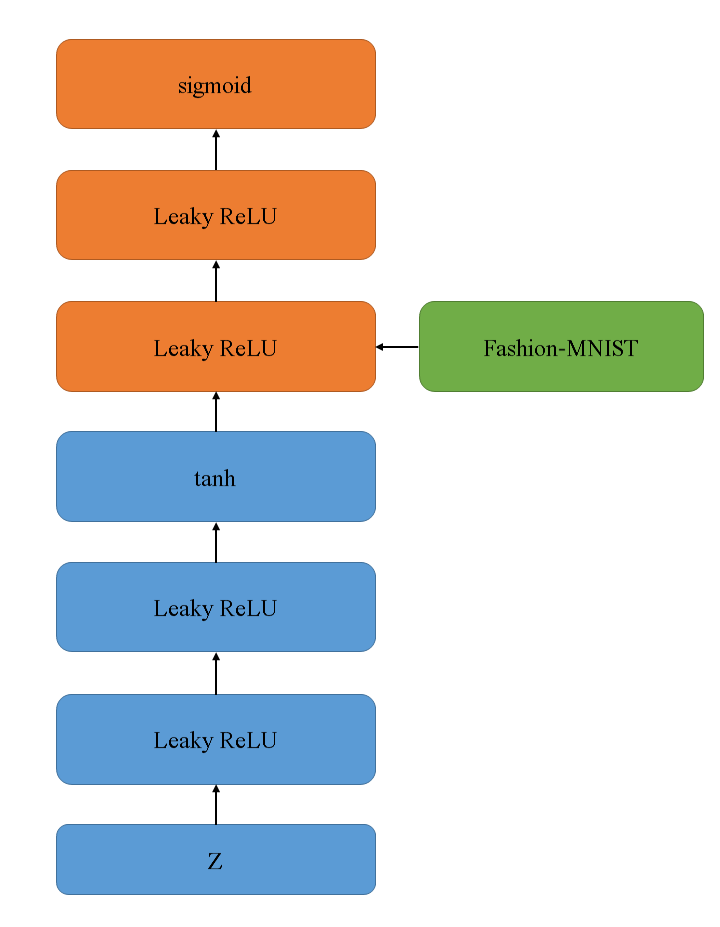
\includegraphics[height=8cm]{gan_network.png}
\caption{GAN Architecture }
\end{figure}

\section{Optimization Algorithm}

In  this study, we use Adaptive Moment Estimation (Adam) optimizer, which is based on the exponentially decaying average of the past gradients. Furthermore, Adam takes advantage of the exponentially decaying average of past gradients $m_i$, similar to momentm method,
$$
m_i = \beta_1 m_{i-1} + (1 - \beta_1) g_i
$$
$$
v_i = \beta_2 v_{i-1} + ( 1- \beta_2 ) g_i^2
$$
$m_i$ and $v_i$ are estimations of the first moment (the mean) and the second moment ( the uncentered variance) of the gradients, respectively. As $m_t$ and $v_t$ are initially close to the vector $0$ ’s, the author of the method have porposed to compute bias-corrected first and second moment estimates using the following equation,
$$\hat{m_i} = \frac{m_i}{( 1- \beta_1^i)}$$
$$\hat{v_i} = \frac{v_t }{( 1- \beta_2 ^i)}$$
The update then applied as follows,
$$
\theta_{i+1} = \theta_i - \frac{\alpha}{   \sqrt{\hat{v_i}}  + \epsilon} \hat{m_i}
$$
The following parameters are chosen for update,
$$
\beta_1 = 0.9, \beta_2 = 0.999,  \textrm{and } & &  \epsilon = 10^{-8}
$$
The optimization for the generator and discriminator vairables are done seperately. 

\end{section}

\section{Result }

In this study, GAN is going to be applied Fashion-MNIST dataset with objective to create a generator with capability to create image of fashion clothes, which include T-shirt/top, trouser, pullover, dress, coat, sandal, shirt, sneaker, bag, and ankle boot. In general, MNIST dataset is so simple, and networks working on this dataset are not necessary capable to real world problems, even with accuracy of 97$\%$ during training and testing. The objective here is to test GAN in a more challenging problem. To do so, neural network is going to be created by TensorFlow by google. 

\end{section}
\section{Conclusion }

In this study, generative adversarial networks are tested on a more complicate dataset (Fashion-MNIST) compared to the MNIST. The Fashion-MNIST dataset includes image of fT-shirt/top, trouser, pullover, dress, coat, sandal, shirt, sneaker, bag, and ankle boot. In general, MNIST dataset is so simple, and networks trined on this dataset do not represent a networks capability as most of the networks get an accuracy of 97$\%$ during training and testing. The objective here is to test GAN in a more challenging problem. To do so, neural network is going to be created by TensorFlow by google. The network also show potential of GAN in Fashion industry for generation of new clothes using convulotional-GAN. The possible objectives are determination of authenticity of a cloth and machine-designed 

\end{section}



%end lec 12
\ifmBIGFILE\else
\bibliographystyle{alpha}
\bibliography{IEEEabrv,bibnotes}
\end{document}
\fi
